\documentclass{beamer}
\usepackage[utf8]{inputenc}
\usepackage[final]{pdfpages}

\usetheme{Goettingen}%Warsaw}
\usecolortheme{lily}
\setbeamertemplate{footline}[page number]
\title[A Case for Scaling Applications to Many-core with OS Clustering ]{A Case for Scaling Applications to Many-core with OS Clustering}
\author{
(reviewed by Oleg Iegorov and Jander Nascimento)}
\institute{University Joseph Fourier}
\date{\today}
\begin{document}

\begin{frame}
\titlepage
\end{frame}

%\AtBeginSubsection[]
{
  \begin{frame}<beamer>
    \frametitle{Roadmap}
    \tableofcontents%[currentsection,currentsubsection]
  \end{frame}
}

%this is filled up with some sample code (we can remove it anytime)

\section{Scaling Operating Systems For Many Cores}

\begin{frame}{Scaling Operating Systems For Many Cores}
  Nowaday's tendencies:
  \begin{itemize}
    \item the number of CPU cores in a system increases;
    \item parallel applications use fine-grained components;
  \newline
  \end{itemize}

  \pause
  \textbf{OS becomes a bottleneck!}
  \newline
  
  \begin{center}
    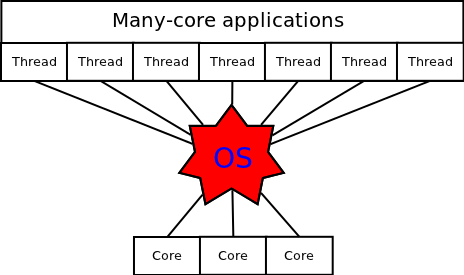
\includegraphics[scale=0.4]{bottleneck.png}
  \end{center}
\end{frame}


\begin{frame}{Scaling Operating Systems For Many Cores}
  Two main approaches:
  \begin{enumerate}
    \item designing new OSes
      \begin{itemize}
        \item distribute independent kernels on multiple cores;
        \item reduce resource sharing \& improve data locality;
      \end{itemize}
    \item refining commodity kernels
      \begin{itemize}
        \item design new data structures to reduce the contention on
          shared data structures;
        \item \emph{interesting fact:} Linux kernel can efficiently scale to 48
          cores!
      \end{itemize}
  \end{enumerate}
\end{frame}

\section{OS clustering approach}

\begin{frame}[t]{OS clustering approach}
  \only<1,2>{
  New approach proposed by this paper: \textbf{OS clustering}
  \begin{itemize}
    \item cluster multiple OSes atop a VMM;
    \item several OSes can serve one application;
  \end{itemize}
  }

  \only<3>{
  \begin{block}{Results}
    \begin{itemize}
      \item single OS manages fewer cores;
      \item resource contention is mitigated.
    \end{itemize}
  \end{block}
  }

  \only<1>{
  \begin{block}{Motivation}
    \begin{enumerate}
      \item commodity kernels scale well with small \# of CPU cores;
      \item one VMM can efficiently consolidate multiple OSes;
    \end{enumerate}
  \end{block}
  }

  \only<2,3>{
    \begin{center}
      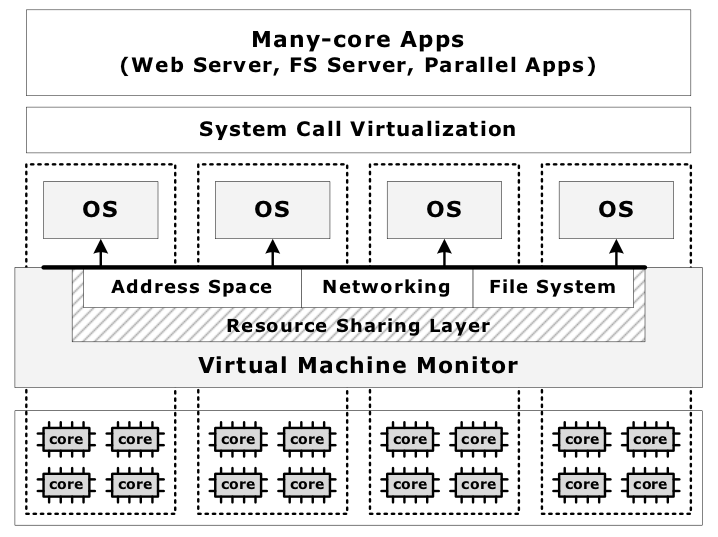
\includegraphics[scale=0.3]{overview.png}
    \end{center}
  }
\end{frame}

\begin{frame}[t]{What's next?}
  The implemented system was called \textbf{Cerberus}
  \newline 

  \begin{itemize}
    \item overview of Cerberus;
    \item more implementation details;
    \item evaluation results
  \end{itemize}
\end{frame}

\section{Overview of Cerberus architecture}

\begin{frame}{Overview of Cerberus architecture}
  \begin{center}
    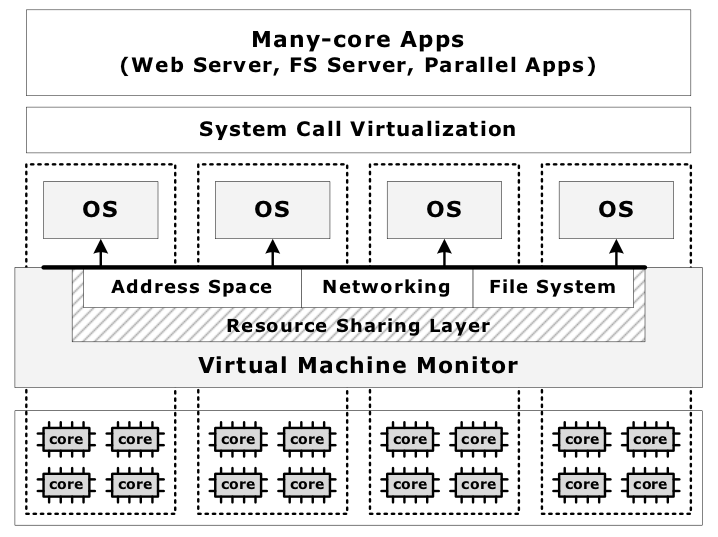
\includegraphics[scale=0.3]{overview.png}
  \end{center}
\end{frame}

\section{System call virtualization}

\begin{frame}[t]{System call virtualization}
  The notion of \textbf{SuperProcess}
  \newline
  \begin{center}
    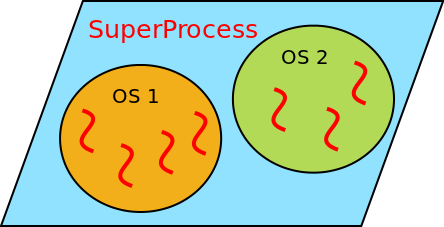
\includegraphics[scale=0.5]{SuperProcess.png}
  \end{center}
\end{frame}

\begin{frame}{System call virtualization}
  Why it is needed?
  \begin{itemize}
    \item all syscalls should be intercepted;
    \item allow processes/threads of one application to run on several
      OSes;
    \item transparent to the user (POSIX API)
  \end{itemize}
\end{frame}

\begin{frame}{System call virtualization}
  \begin{center}
    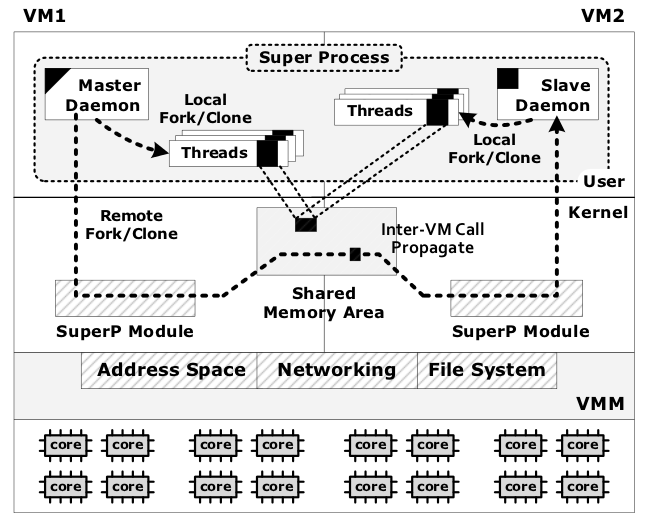
\includegraphics[scale=0.4]{adv_architecture.png}
  \end{center}
\end{frame}

\section{Resource Sharing}

\begin{frame}{Resource Sharing}
  \begin{itemize}
    \item processes/threads of one application must share some
      resources;
    \item VMMs are designed to isolate VMs from each other;
    \item \emph{resource sharing layer} must modify VMM's code
  \end{itemize}
  \begin{center}
    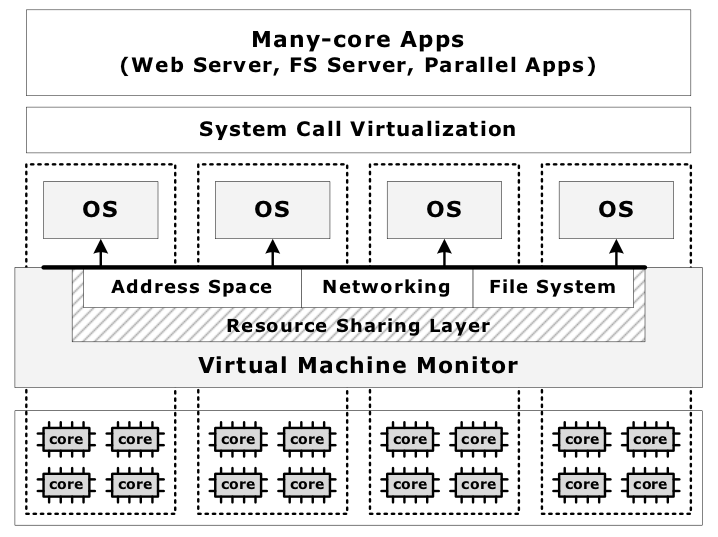
\includegraphics[scale=0.3]{overview.png}
  \end{center}
\end{frame}


\section{Process management}

	\begin{frame}[plain]
		\begin{figure} [H]
			\centering
			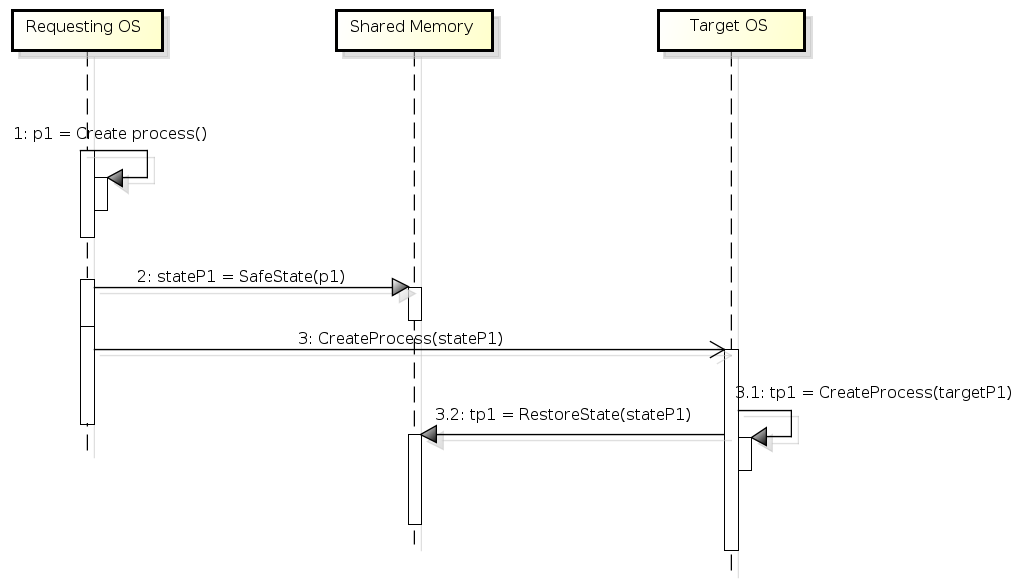
\includegraphics[scale=0.46]{img/cerberus-process-creation}
		\end{figure}
	\end{frame}

	\begin{frame}{Remote process}

	\begin{figure} [H]
			\centering
			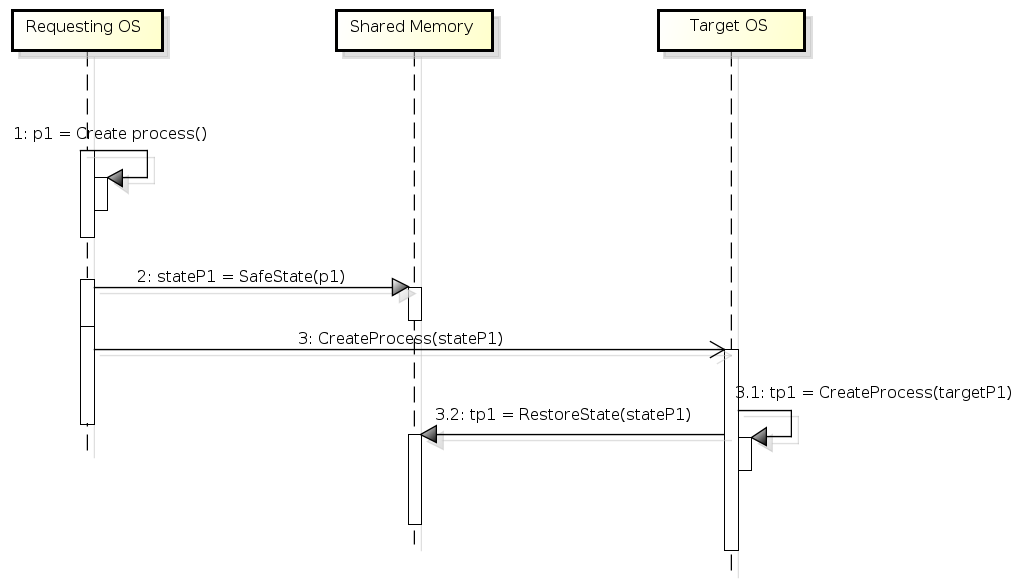
\includegraphics[scale=0.3]{img/cerberus-process-creation}
	\end{figure}

	\begin{itemize}[<+->]
	\item Create local process
	\item Saves the state of the process
	\item Request target OS to create a process
	\item Target OS restores the state
	\end{itemize}
	
	\end{frame}	
	
	\begin{frame}{Fork and Clone}
	
		\begin{figure} [H]
			\centering
			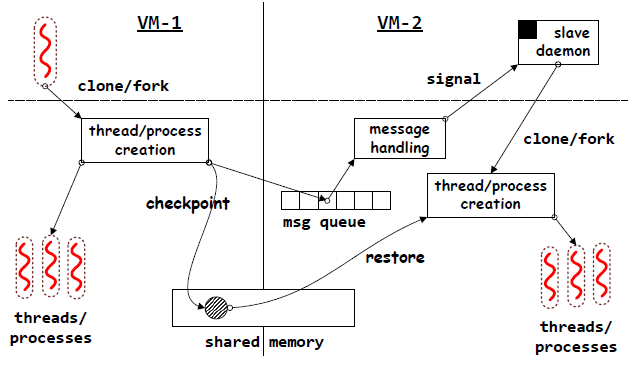
\includegraphics[scale=0.40]{img/cerberus-fork-clone}
		\end{figure}	
	
	\end{frame}	
	
	\begin{frame}{Turn into reality}

	Main changes?	
	\begin{itemize}
	\item Syscall intercept	
	\item Virtualized PID
	\item Compare and swap to access page table
	\item Address range abstraction
	\end{itemize}
	
	Examples?
	\begin{itemize}
	\item Kill
	\item Futex call
	\item Set affinity
	\end{itemize}	
	
	\end{frame}

	\begin{frame}{Syscall virtualization}
	
		\begin{figure} [H]
			\centering
			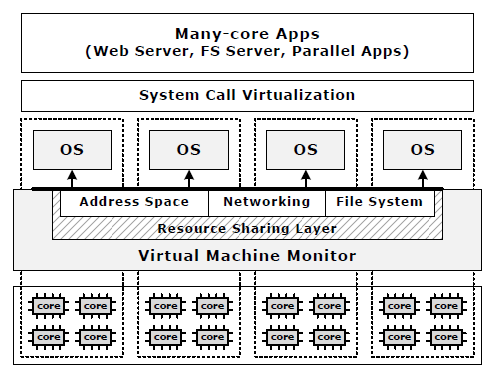
\includegraphics[scale=0.40]{img/syscall-virtualization}
		\end{figure}	

	\end{frame}
	
	\begin{frame}{Shared Data Segment}
	
	Multiprocess application	
	
	\begin{itemize}	
		\item Not common share data
	\end{itemize}	
	
	Multi-threaded application:
	
	\begin{itemize}		
	\item Process table
	\item File descriptor table
	\end{itemize}
	
	\end{frame}

%	\begin{frame}{Cerberus arch}
%
%		\begin{figure} [H]
%			\centering
%			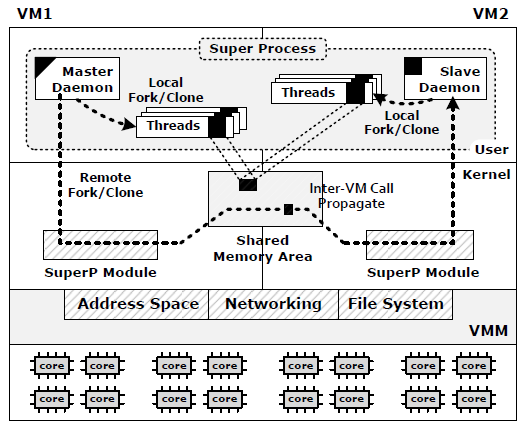
\includegraphics[scale=0.40]{img/cerberus-architecture}
%		\end{figure}	
%
%	\end{frame}

\section{Sharing file}
	
	\begin{frame}{Sharing file}	
	
		Use existent network file systems:
		\begin{itemize}
		\item NFS
		\end{itemize}
		
		Issues?
		\pause 
		
		\begin{itemize}
		\item Centralized
		\item Rather slow
		\end{itemize}		

	\end{frame}	
	
	\begin{frame}{Sharing file}	
	
		\begin{block}{Solution?}
			Use remote and local file access
		\end{block}
		
		In another perspective:		
		\begin{itemize}
		\item Hybrid solution: local and remote file access.
		\item Basic security scheme: public or private file.
		\end{itemize}

	\end{frame}

	\begin{frame}{CFS arch}

		\begin{figure} [H]
			\centering
			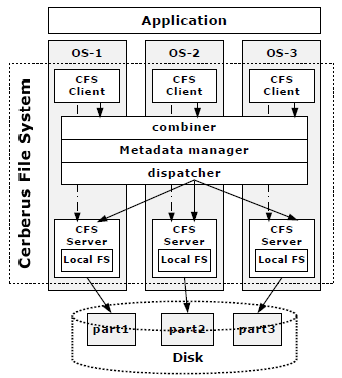
\includegraphics[scale=0.45]{img/cerberus-cfs}
		\end{figure}	

	\end{frame}

\section{Evaluation}

	\begin{frame}{Evaluation environment}

	Hardware overview
	
	Configuration 1:
	\begin{itemize}
	\item AMD 48 cores (8 x 6-cores) 
	\item 4 network cards
	\end{itemize}	

	Configuration 2:
	\begin{itemize}
	\item Intel Quadcore 4 cores
	\item 8 network cards
	\end{itemize}	
	\end{frame}

	\begin{frame}{Stepping stone}
	
	Tech overview:
	\begin{itemize}
	\item based on Xen
	\item POSIX calls re-implemented
	\end{itemize}

	All performance measurements repeated at least 3x

	\end{frame}

	\begin{frame}{Sending signals}

		Result of ping-ponging signals:
		
		\begin{tabular}{|c|c|c|}
		\hline Case & Intel & AMD \\ 
		\hline Native Linux & 7.9ms & 4.0ms \\ 
		\hline Xen-Linux & 38.7ms & 74.1ms \\ 
		\hline Cerberus local & 43.1ms & 72.3ms \\ 
		\hline Cerberus remote & 25.8ms & 45.0ms \\ 
		\hline 
		\end{tabular} 
	
	\end{frame}
	
	\begin{frame}{Fork}

		Forking remotely:		
		
		\begin{tabular}{|c|c|c|}
		\hline Primitive & Config & Time \\ 
		\hline remote fork & 1 process & 5.40ms \\ 
		\hline remote fork & 24 process & 31.77ms \\ 		
		\hline 
		\end{tabular} 

	\end{frame}
	
	\begin{frame}{WebServer}
	
		Testing Cerberus as a virtualized WebServer
	
		\begin{figure} [H]
			\centering
			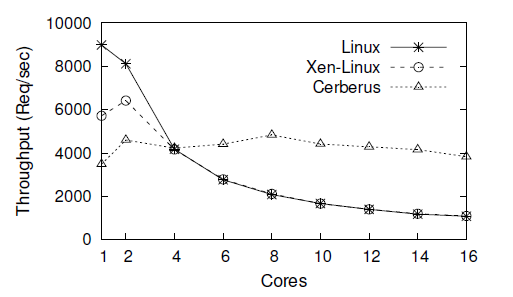
\includegraphics[scale=0.60]{img/cerberus-webserver}
		\end{figure}		
	
	\end{frame}	
	
\section{Our evaluation}

	\begin{frame}{Downside}

	Some negative points of the paper:
	\begin{itemize}
	\item Do not show the performance of CFS in operations like: writing and seeking
	\item Do not explain how solve the problem of centralization for load balance
	\item Do not show the numbers for acceptable performance
	\item Tested on a System with only 48 cores
	\item Code is not available
	\end{itemize}

	\end{frame}

\section{That is it}

	\begin{frame}{}

	\begin{alertblock}{Thanks for the patience}
	Question?
	\end{alertblock}

	\end{frame}

\end{document}
